\section{Kältetechnischer Aufbau}
\label{sec: Kältetechnischer Aufbau}

In diesem Abschnitt werden die Teilsysteme des kältetechnischen Aufbaus vorgestellt. Der komplette kältetechnischer Aufbau besteht aus der Kälteanlage(KA) mit dem Verdampfer-Prüfling und der Klimakammer(KK), in der der Prüfling lokalisiert ist und unter verschiedenen Umgebungsgebenheiten getestet werden kann.

\subsubsection{Kälteaanlage(KA)}
\label{subsec:Kälteanlage}



Die Auslegungsdaten der KA sind in Tabelle \ref{tab:Parameter KK} dargestellt. In Abbildung \ref{fig:KA-Fliessbild}  ist das Fließschema der KA dargestellt. 



\begin{table}[htb]
\centering
\caption{Leistungsdaten Kälteanlage}\vspace{6pt}
\label{tab:Parameter KK}
\begin{tabular}{cc}
\hline 
\textbf{Systemparameter} & \textbf{Kälteanlage(KA)} \\ 
\hline 
\hline
Kältemittel & R134a\\
\hline
Verdampfungstemperatur & -8,0 $°C$\\
\hline
Verdampfungsdruck(abs) & 2,17 Bar\\
\hline
Verflüssigungstemperatur & 40,2 $°C$\\
\hline
Verflüssigungsdruck(abs) & 10,23 Bar\\
\hline
Sauggastemperatur & 2 $°C$\\
\hline
Verdichtungstemperatur &72,4 $°C$\\
Kälteleistung & 11,2 kW \\ 
\hline 
Verflüssigungsleistung & 15,3 kW\\
\hline
Leistungsaufnahme & 4,07 kW \\ 
\hline
Kälteleistungszahl & 2,74\\
\hline 
Massenstrom & 0,077 kg/s \\ 
\hline 
max. Leistung der Lufterwämer & 2x 20 kW \\ 
\hline 
max. Befeuchtungsleistung & 12 g/h \\ 
\hline 
max. Kühlleistung & 10 kW \\ 
\hline 
min. Temperatur & 16,3 $°c$ \\ 
\hline 
Steuer- und Regelungstechnik & TWINCAT 3/ VB.NET \\ 
\hline 
Hart echtzeitfähig & Ja \\ 
\hline 
\end{tabular} 
\label{tab:KA-Auslegungsdaten}
\end{table}

Die Hauptkomponenten der Kälteanlage sind der Kompressor, der Verflüssiger, der Verdampfer und der Abtau-Verdampfer. Der Verflüssiger kondensiert im  Kühlbetrieb das überhitzte Kältemittel vollständig und der Abtauverdampfer verdampft das Kältemittel im Abtaubetrieb durch Prozessumkehrung, bevor es zurück in den Kompressor gesaugt wird. Der Verdampfer ist gleichzeitig der Prüfling, den es zu untersuchen gilt. Der Verdampfer ist durch die vorgesehenen Absperrventile austauschbar. Diese Vorrichtung ermöglicht unterschiedliche Bautypen von Verdampfer zu testen. 

Zwischen den Zustandspunkten 1 und 2 erfolgt die Verdichtung und Überhitzung des Kältemittels. Danach gelangt das Kältemittel in den Ölabscheider, der einen großen Teil des Öls vom Kältemittel trennt und zurück zur Schmierung des Verdichters führt. Vor und nach dem Kompressor sind sowohl zur Energie-Bilanzierung als auch zwecks Anlagenschutz Temperatur- und Drucksensoren installiert. Dieser Vorgang ist im Abtau- und Kühlbetrieb identisch. 

Das Kältemittel, das aus dem internen Wärmeübertrager Richtung Kompressor gesaugt wird, passiert zunächst den Tropfenabscheider.  Der Tropfenabscheider stellt sicher, dass kein noch flüssiges Kältemittel in den Kompressor eindringt. Dies hätte verheerende Folgen für den Kompressor und wird genauer in Abschnitt \ref{subsec: Anlagenschutz} des Anlagenschutzes beschrieben. 

In der KK findet der Verdampfungsprozess statt. Neben dem Verdampfer ist hier das Expansionsventil und die Versorgungsmimik installiert. Die Versorgungsmimik erlaubt 3 verschiedene Durchströmungswege durch den Verdampfer. Die Abbildung \ref{fig:Magnetventil} sind die Varianten mit den Magnetventilstellungen abgebildet. 

\begin{figure}[htb]
%\centering	
\includegraphics[ page=4, width=1.150\textwidth]{Pictures/RI.pdf}
\caption{Kälteanlage(KA)-Fließbild}
\label{fig:KA-Fliessbild}
\end{figure}

\subsubsection{Kühlbetrieb, Zustandspunkte: $1 \rightarrow 2 \rightarrow 2'\rightarrow 3' \rightarrow 3''\rightarrow  3''' \rightarrow 3 \rightarrow 4 \rightarrow 1' $}

Im Kühlbetrieb strömt das flüssige, unterkühle Kältemittel nach dem Verflüssiger erst in den Sammler. Danach überträgt es Wärme zwischen den Zustandspunkten $3''$ und $3'''$ an das aus dem Verdampfer kommende verdampfte Kältemittel. Am Zustandspunkt $3$ befindet sich der Massenstromsensor und ein Schauglas.  
Im \textbf{Kühlbetrieb} wird das Kältemittel durch das Expansionsventil entspannt und nochmal kurz vor dem Verdampfer durch eine Venturidüse ein weiteres Mal entspannt und eingespritzt.

\subsubsection*{Abtaubetrieb, Zustandspunkte: $1 \rightarrow 2 \rightarrow 1'\rightarrow 4 \rightarrow 3''\rightarrow  3''' \rightarrow 3 \rightarrow 3' \rightarrow 2' $}

Im Abtaubetrieb durch Prozessumkehrung fließt das Kältemittel, vom Verdampfer kommend, auch erst in den Sammler, um danach durch den internen Wärmeübertrager zum Massenstromsensor zu gelangen. Danach wird es über das Expansionsventil in den Abtau-Verdampfer eingespritzt. Rückschlagventile sind jeweils vor und nach einem Wärmeübertrager installiert. Rückschlagventile erlauben dem Kältemittel nur in eine Richtung zu fließen. Dies ermöglicht, dass im Abtaubetrieb das Kältemittel durch den Abtauverdampfer geführt wird und dort verdampft. 

Im Abtaubetrieb durch Prozessumkehrung kann das Heißgas entweder durch die Venturidüse in den Verdampfer gelangen oder durch die Saugleitung \footnote{In dem weiteren Verlauf der Arbeit wird von Heißgaseintritt über die Venturidüse von \textit{Oben} gesprochen, da der Wärmeübertrager aus 4 Rohrlamellen-Wärmeübertrager besteht und die Einspritzung stets im obersten,rechten  Rohr geschieht. Von \textit{Unten} wird hingegen benutzt um die Variante mit Eingang des Heißgases über die Saugleitung zu beschreiben, da die Saugleitung stets das unterste Rohr ist.}.  






%\footnote{Mit Abtaubetrieb ist hier nur die Abtaumethode Prozessumkehrung gemeint. Bei der elektrischen Abtauung steht die Kältemaschine still und fährt erst nach dem Abtauprozess wieder an.} 



\begin{figure}%[htb]
\centering		
\hspace{2cm}\includegraphics[page={3},width=1.15\textwidth]{Pictures/Schaltschema.pdf}
\caption{Mögliche Magnetventil-Schaltungen}
\label{fig:Magnetventil}
\end{figure}

\subsubsection*{Messtechnik}
\label{subsubsec:Messtechnik}

Die KA ist ausgerüstet mit drei Sensorenarten: Temperatur-, Druck- und Massenstromsensoren. Diese Sensoren dienen zur Bilanzierung der Wärmeübertrager und des Kompressors, spielen aber auch eine wichtige Rolle beim Anlagenschutz. In Tabellen \ref{tab:Messtechnik KA} sind die Sensordaten aufgeführt. 



\begin{table}[htb]
\centering
\caption{Sensordaten-Übersicht}\vspace{6pt}
\label{tab:Messtechnik KA}
\begin{tabular}{p{3cm}p{3cm}p{3cm}p{3.5cm}llll}
\hline 
 & \textbf{Drucksensor} & \textbf{Temperatursensor} & \textbf{Massenstromsensor} \\ 
\hline 
\hline 
Typ & PA 33 X & • & OPTIMASS 6400 C \\ 
\hline 
Hersteller & KELLER AG & • &  KROHNE Messtechnik GmbH \\ 
\hline 
Messbereich & 0..30 Bar(0..10 Bar) & • & 0..400 kg/h \\ 
\hline 
Messfehler[$\%$] & 0,01 (10..40$°C$)\newline 0,1(-10..80$°C$) & 0,1  & 0,6 \\ 
\hline 
Komunikationsart & RS-485 & 4..20 mA & RS-485 \\ 
\hline 
Abfragefrequenz & 400 Hz & • & • \\ 
\hline 
Hilfsenergie [V] & 8..28 & - & 230  \\ 
\hline
Anzahl & 8  & 11 & 1 \\ 
\hline 
%Datenblatt(URL) & http://www.keller-druck.com/picts/pdf/german/33xg.pdf & • & https://www.instrumart.com/assets/Krohne-optimass6000-datasheet.pdf \\ 
\hline 
\end{tabular} 
\label{tab:Tabelle}
\end{table}

\newpage
\subsubsection{Klimakammer(KK)}
\label{subsec:Klimakammer}
\begin{figure}[htb]
\centering		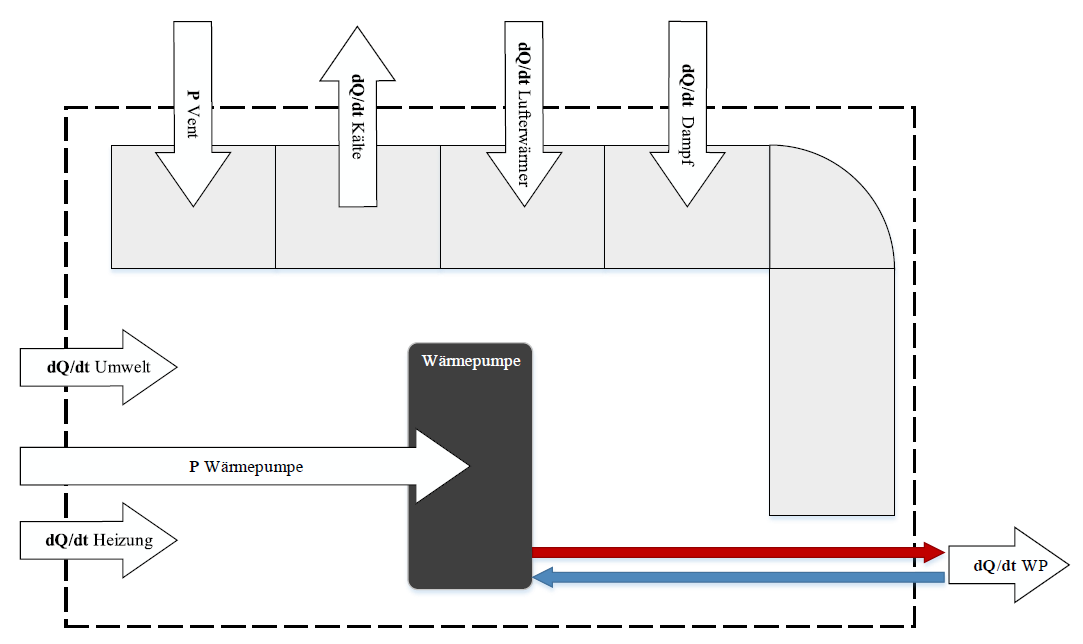
\includegraphics[width=0.850\textwidth]{Pictures/HIL2.png}
\caption{Wärmeströme in der Klimakammer \citep{Nuerenberg2015}}
\label{fig:KK}
\end{figure}


Die KK erlaubt es den Verdampfer und somit den Vereisungs- und Abtauprozess unter verschiedenen Abtaubedingungen zu untersuchen. Die KK ist als klassisches \textit{Hardware in the Loop} Die Kenndaten der KK sind in Tabelle \ref{tab:Parameter KK}. Die Abbildung \ref{fig:KK} zeigt die Wärmeströme innerhalb der KK. Die KK ist in der Lage eine stationäre Umgebungsbedingungen abzubilden. Es ist aber auch möglich instationäre Situationen wie zum Beispiel Typtage oder -wochen nachzustellen. 
In der KK ist die Verdampfereinheit mit der Kältemittelversorgungs-Mimik lokalisiert. Des Weiteren ist das Wägesystem und die eingesetzten Waagen in der KK plaziert. 



Die KK ist konzipiert für  Untersuchungen von Wärmepumpen und Kältemaschinen. Der Einsatz der KK in Kombination mit einer klimatisierbaren Versuchshalle hebt die Reproduzierbarkeit von Messungen. Die Bedingungen für Versuche können unabhangig von der Jahreszeit oder dem Tagesklima konstant gehalten werden. So lassen sich Versuche mit verschiedensten Umgebungsbedingungen ganzjährlich durchführen.  Die einzustellen Parameter sind die Temperatur und die Relative Luftfeuchtigkeit($RH$). Die KK wurde 2015 in Betrieb genommen und wird wie die KA auch über eine SPS der Fa. Beckhoff geregelt und gesteuert. In dem KK-Projekt wurde von \textsc{\citeauthor{Nuerenberg2015}} beispielsweise die $Status Maschine$ eingeführt, auf der auch das Konzept der SPS der KA beruht, siehe Abschnitt \ref{sec:Informationstechnischer Aufbau}. 

Die KK verfügt über Software-Schnittstellen  mit Simulationssoftwares (zB. \textsc{Dymola}) und Datenbanken (zB. \textsc{MySQL}). Die Kombination aus Simulator mit echter Hardware wird als \textit{Hardware in the Loop} bezeichnet. Diese Methode dient zum Testen und Absichern von eingebetteten Systemen, die noch in der Entwicklung sind oder sich in der Inbetriebnahme befinden. Die Vorteile dieser Methode liegt in der Verkürzung der Inbetriebnahmephase, Verringerung der Entwicklungskosten und das riskofreie Testen der Anlage in Grenzsituationen. \citep{OPALRTT2014}


\begin{table}[htb]
\centering
\caption{Systemparamter der Klimakammer \citep{Nuerenberg2015}}\vspace{6pt}
\label{tab:Parameter KK}
\begin{tabular}{lc}
\hline 
\textbf{Systemparameter} & \textbf{Klimakammer(KK)} \\ 
\hline 
\hline
Volumen & 32,96 m$^3$ \\ 
\hline 
Oberfläche & 74,4 m$^2$ \\ 
\hline 
Wandstärke & 0,15 m \\ 
\hline 
max. Volumenstrom & 4000 m$^3$/h \\ 
\hline 
max. Leistung der Lufterwämer & 2x 20 kW \\ 
\hline 
max. Befeuchtungsleistung & 12 g/h \\ 
\hline 
max. Kühlleistung & 10 kW \\ 
\hline 
min. Temperatur & 16,3 $°c$ \\ 
\hline 
Steuer- und Regelungstechnik & TWINCAT 3/ VB.NET \\ 
\hline 
Hart echtzeitfähig & Ja \\ 
\hline 
\hline
\end{tabular} 
\label{tab:Systemparameter-KK}
\end{table} 

